% fs-11-Correlation.tex

\documentclass[xcolor=dvipsnames]{beamer}
\usepackage{teachbeamer}

\title{Correlation}
\subtitle{{\CourseNumber}, BCIT}

\author{\CourseName}

\date{April 19, 2018}

% \begin{figure}[h]
% 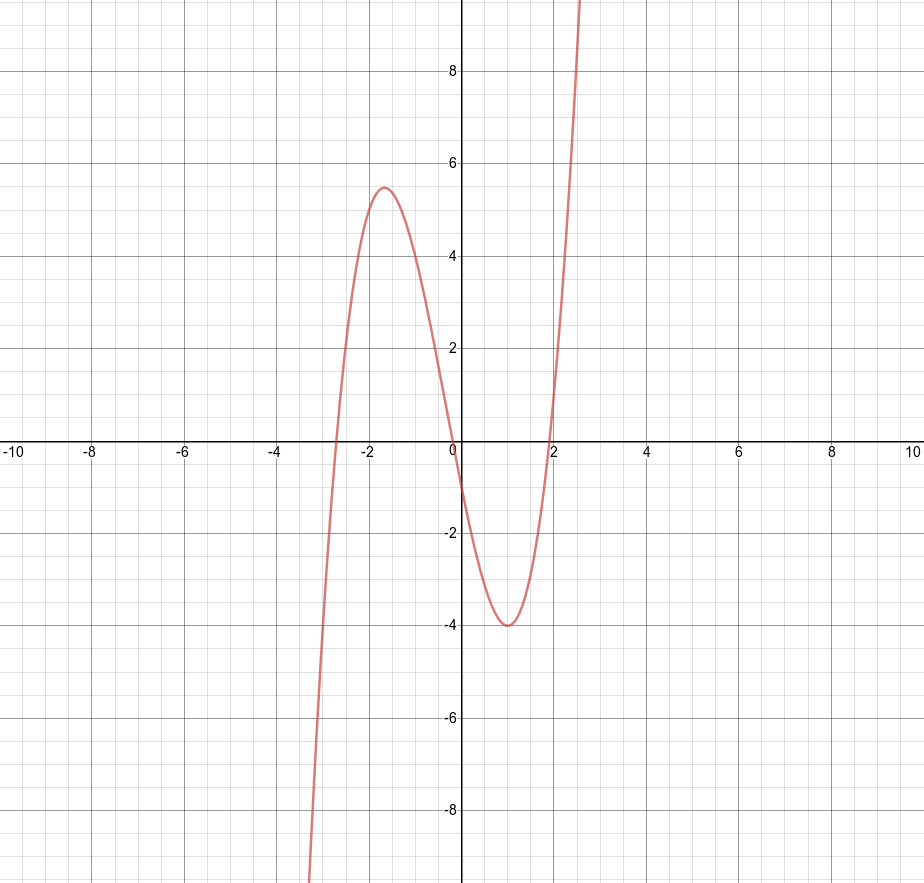
\includegraphics[scale=.3]{./diagrams/extrema1.png}
% \end{figure}

% Command             10pt    11pt    12pt
% \tiny               5       6       6
% \scriptsize         7       8       8
% \footnotesize       8       9       10
% \small              9       10      10.95
% \normalsize         10      10.95   12

\begin{document}

\begin{frame}
  \titlepage
\end{frame}

% \begin{frame}
%   \frametitle{Instructor Note}
%   I want to change this from emphasis on correlation coefficients and
%   using the critical values on the Pearson correlation coefficient
%   table to doing a proper hypothesis test for the slope $b_{1}$ with a
%   null hypothesis $\beta_{1}=0$. This way you can find a confidence
%   interval for $\beta_{1}$ and a prediction interval for $\hat{y}$
%   (see Devore and Peck's textbook); and the integration with R
%   Statistics is much better. There is also a natural segue to ANOVA
%   with the F-test in R Statistics on linear correlation. Course
%   Outline wants both. It also wants you to do the Kolmogorov-Smirnoff
%   test for normality.
% \end{frame}

\begin{frame}
  \frametitle{Correlation}
  A \alert{correlation} exists between two variables when the values of
  one variable are somehow associated with the values of the other
  variable.

  \bigskip

    A \alert{linear correlation} exists between two variables when
    there is a correlation and the plotted points of paired data
    result in a pattern that can be approximated by a straight line.
\end{frame}

\begin{frame}
  \frametitle{Correlation}
  Here is the data for waist (in inches), weight (in pounds), and body
  fat (in percent) for 20 test subjects.

% barney/teaching/courses/MATH2441/deveau-velleman-bock/De Veaux_Velleman_Bock Datasets/SDM4e_Datasets/Chapter_25/CSV Data Files/Body_fat.csv
% 33,188,10,,33,160,10,,40,192,31,,32,175,6
% 40,240,20,,41,215,27,,41,205,32,,36,181,21
% 36,175,22,,34,159,12,,35,173,21,,38,200,15
% 32,168,9,,34,146,10,,38,187,25,,33,159,6
% 44,246,38,,44,219,28,,38,188,30,,39,196,22

\begin{alltt}
\scriptsize
+---+---+--++---+---+---++---+---+---++---+---+--+\newline
| 33|188|10|| 33|160| 10|| 40|192| 31|| 32|175| 6|\newline
+---+---+--++---+---+---++---+---+---++---+---+--+\newline
| 40|240|20|| 41|215| 27|| 41|205| 32|| 36|181|21|\newline
+---+---+--++---+---+---++---+---+---++---+---+--+\newline
| 36|175|22|| 34|159| 12|| 35|173| 21|| 38|200|15|\newline
+---+---+--++---+---+---++---+---+---++---+---+--+\newline
| 32|168| 9|| 34|146| 10|| 38|187| 25|| 33|159| 6|\newline
+---+---+--++---+---+---++---+---+---++---+---+--+\newline
| 44|246|38|| 44|219| 28|| 38|188| 30|| 39|196|22|\newline
+---+---+--++---+---+---++---+---+---++---+---+--+
\end{alltt}
\end{frame}

\begin{frame}
  \frametitle{Correlation}
\begin{figure}[h]
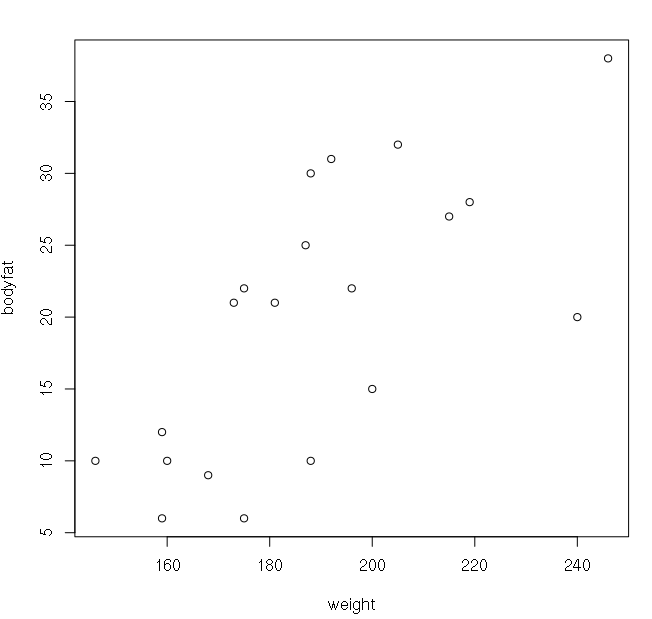
\includegraphics[scale=.35]{./diagrams/bf-01.png}
\end{figure}
\end{frame}

\begin{frame}
  \frametitle{Correlation}
  In the previous slide, you can see the data from 20 test subjects.
  In the following slide, you can see the data from 250 test subjects. It appears that there is a
  relationship between waist and body fat.
\end{frame}

\begin{frame}
  \frametitle{Correlation}
\begin{figure}[h]
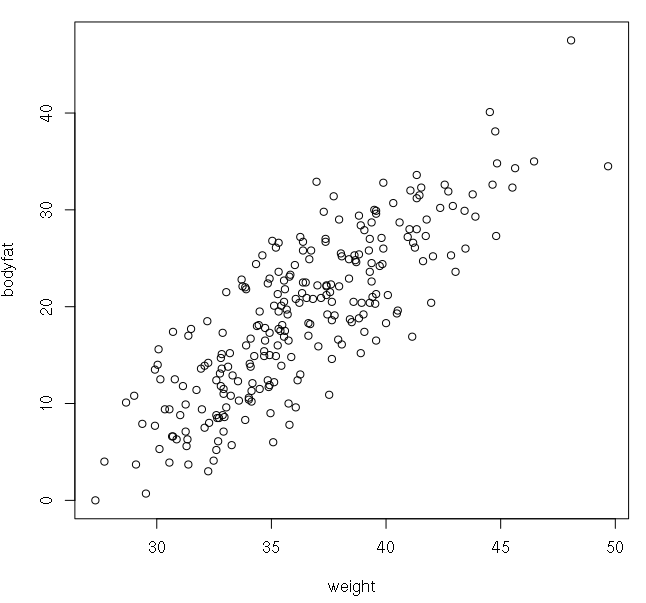
\includegraphics[scale=.35]{./diagrams/bf-02.png}
\end{figure}
\end{frame}

\begin{frame}
  \frametitle{Correlation}
\begin{figure}[h]
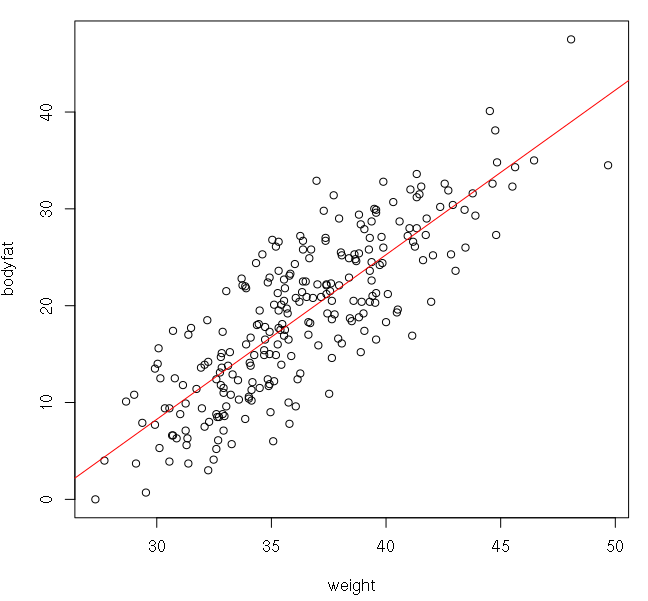
\includegraphics[scale=.35]{./diagrams/bf-03.png}
\end{figure}
\end{frame}

\begin{frame}
  \frametitle{Correlation}
  The red line is called the regression line. We will learn how to
  calculate it later. Here is its equation:
\begin{equation}
  \label{eq:chuitohf}
  b=1.7w-42.73
\end{equation}
The regression line minimizes the mean square distance of the data
points to the line (all other lines have a greater mean square
distance from the data points). Have a look at three of the 250 test
subjects.

\begin{tabular}{|l|r|r|r|r|}\hline
                 & waist & bf (act) & bf (pred) & error   \\ \hline
  test subject 1 & 33.54 & 12.3     & 14.29     & 1.9936  \\ \hline
  test subject 2 & 32.68 & 6.1      & 12.82     & 6.7212  \\ \hline
  test subject 3 & 34.61 & 25.3     & 16.10     & -9.1993 \\ \hline
\end{tabular}
\end{frame}

\begin{frame}
  \frametitle{Correlation}
  It appears that the error is normally distributed (perhaps not quite
  on the margins).
% hist(bfc[[16]],main="histogram of error",xlab="error",breaks=seq(-13,12,2))
\begin{figure}[h]
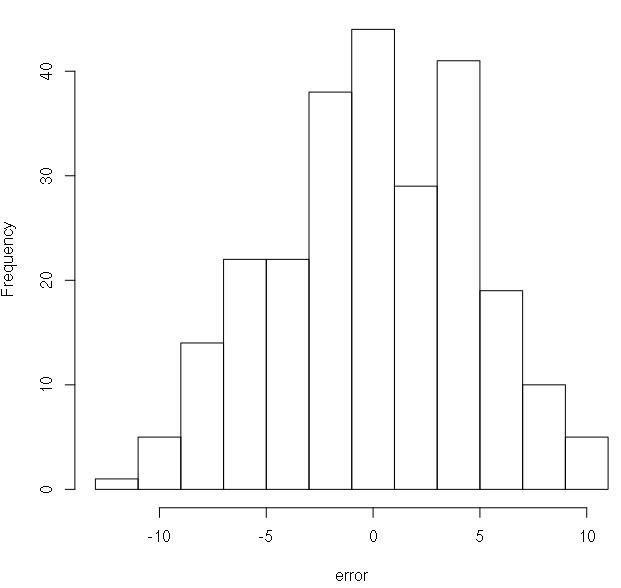
\includegraphics[scale=.3]{./diagrams/bf-04.png}
\end{figure}
\end{frame}

\begin{frame}
  \frametitle{Correlation}
\begin{figure}[h]
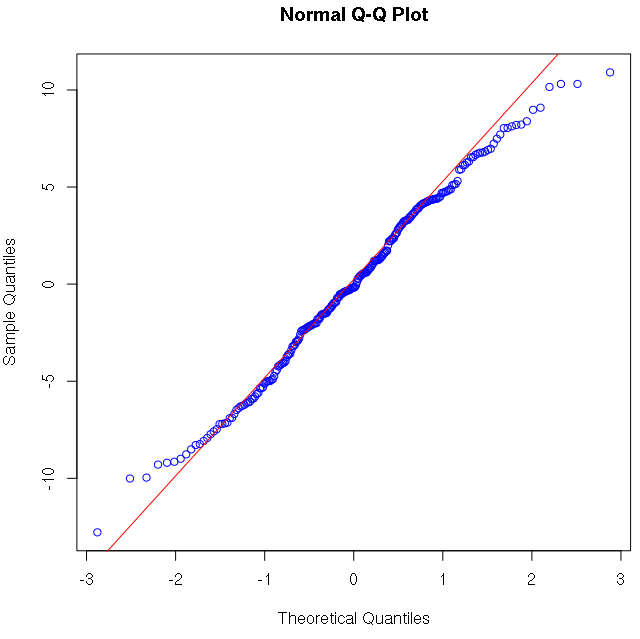
\includegraphics[scale=.35]{./diagrams/bf-05.png}
\end{figure}
\end{frame}

% \begin{frame}
%   \frametitle{Correlation}
%   Have a look at the following table:

%   \bigskip

%   \begin{tabular}{|l|l|l|}\hline
%     \textbf{Subject} & \textbf{Shoe Print} & \textbf{Height} \\ \hline
%     Male 1 & 29.7cm & 175.3cm \\ \hline
%     Male 2 & 29.7cm & 177.8cm \\ \hline
%     Male 3 & 31.4cm & 185.4cm \\ \hline
%     Male 4 & 31.8cm & 175.3cm \\ \hline
%     Male 5 & 27.6cm & 172.7cm \\ \hline
%   \end{tabular}

%   \bigskip

%   Is there a correlation between the two variables?
% \end{frame}

% \begin{frame}
%   \frametitle{Correlation}
%   Here is a scatterplot of 19 males, showing their height ($y$-axis)
%   and their shoe print ($x$-axis).
%   \begin{figure}[h]
%     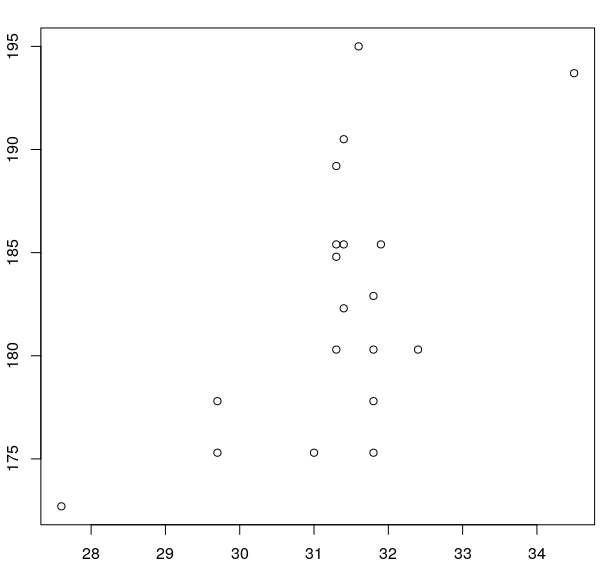
\includegraphics[scale=0.35]{./diagrams/mshoeprintheight.png}
%   \end{figure}
% \end{frame}

% \begin{frame}
%   \frametitle{Correlation}
%   Here is a scatterplot of 21 females, showing their height ($y$-axis)
%   and their shoe print ($x$-axis).
%   \begin{figure}[h]
%     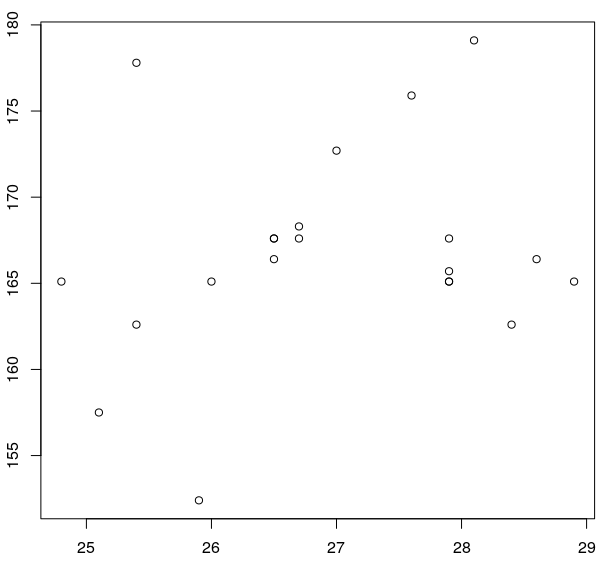
\includegraphics[scale=0.35]{./diagrams/fshoeprintheight.png}
%   \end{figure}
% \end{frame}

% \begin{frame}
%   \frametitle{Correlation}
% Here is the combined scatterplot.
%   \begin{figure}[h]
%     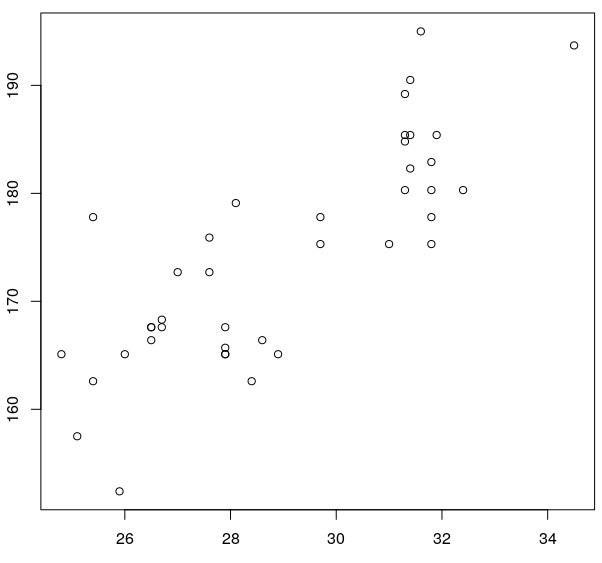
\includegraphics[scale=0.35]{./diagrams/mfshoeprintheight.png}
%   \end{figure}
% \end{frame}

\begin{frame}
  \frametitle{Correlation}
  Let's have a look at a few scatterplots. Is there a correlation or
  not? Is there a linear correlation? The \alert{linear correlation
    coefficient} $r$ measures the strength of the linear correlation.
  It is a sample statistic. The linear correlation coefficient for the
  population is called $\varrho$ (``rho'' in the Greek alphabet).

  \bigskip

  The correlation coefficient for the sample of 250 test subjects
  measuring body fat and waist is $r=0.8236847$.
\end{frame}

\begin{frame}
  \frametitle{Scatterplot Examples}
  \begin{figure}[h]
    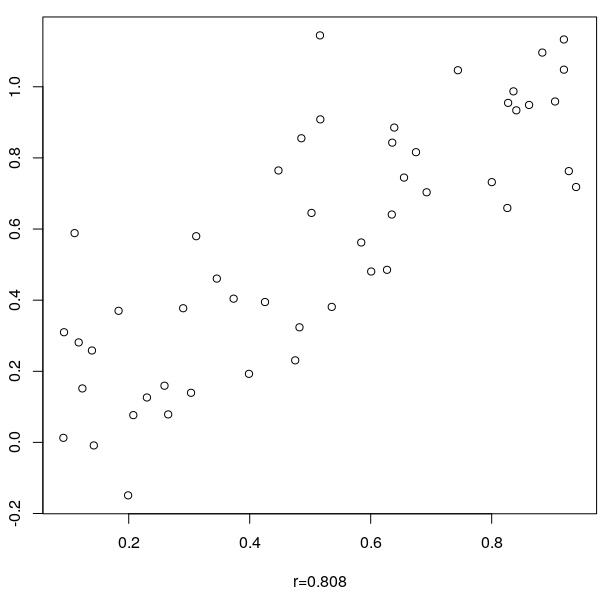
\includegraphics[scale=0.35]{./diagrams/sc01.png}
  \end{figure}
\end{frame}

\begin{frame}
  \frametitle{Scatterplot Examples}
  \begin{figure}[h]
    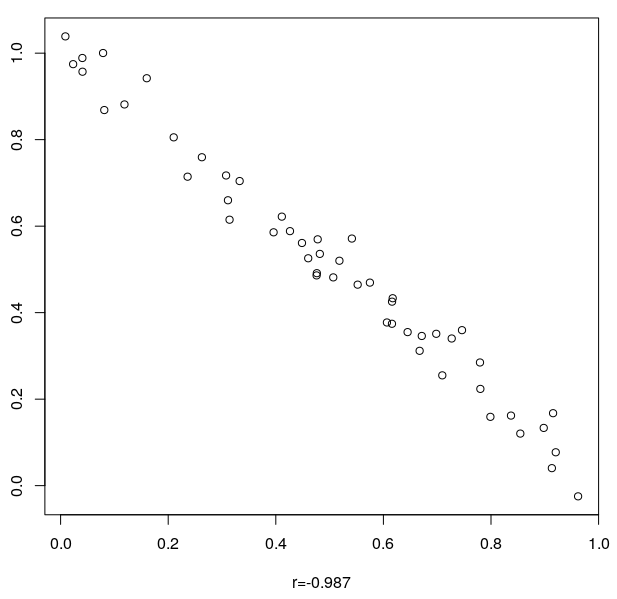
\includegraphics[scale=0.35]{./diagrams/sc02.png}
  \end{figure}
\end{frame}

\begin{frame}
  \frametitle{Scatterplot Examples}
  \begin{figure}[h]
    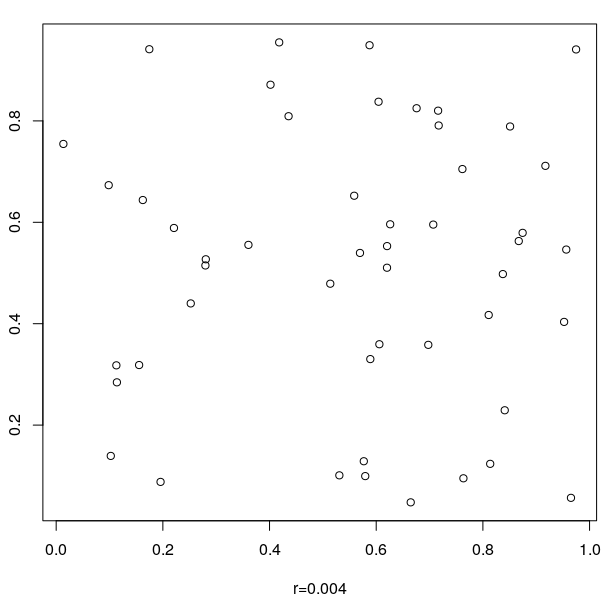
\includegraphics[scale=0.35]{./diagrams/sc03.png}
  \end{figure}
\end{frame}

\begin{frame}
  \frametitle{Scatterplot Examples}
  \begin{figure}[h]
    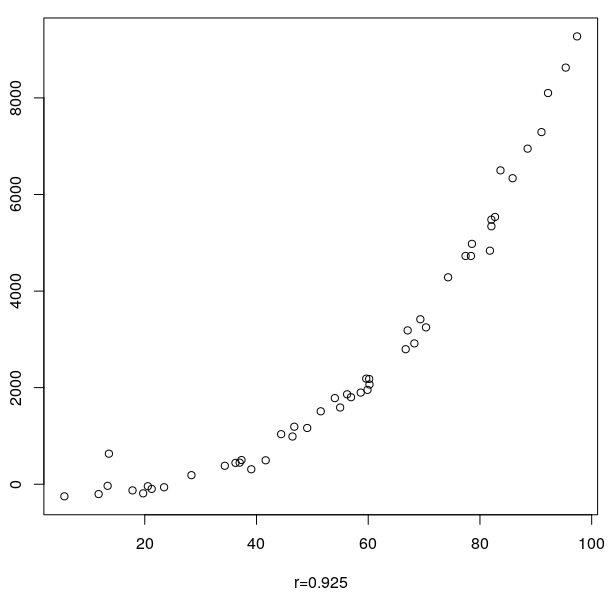
\includegraphics[scale=0.35]{./diagrams/sc04.png}
  \end{figure}
\end{frame}

\begin{frame}
  \frametitle{Notation}
  To determine whether there is a linear correlation between two
  variables, first take note of the following notation.
  \begin{description}
  \item[$n$] number of pairs of sample data
  \item[$\sum$] denotes addition of items indicated
  \item[$\sum{}x$] sum of all $x$-values
  \item[$\sum{}x^{2}$] sum of all $x^{2}$-values
  \item[$(\sum{}x)^{2}$] sum of all $x$-values squared
  \item[$\sum{}xy$] sum of all $x\cdot{}y$-values
  \item[$r$] linear correlation coefficient for sample data
  \item[$\varrho$] linear correlation coefficient for population of paired data
  \end{description}
\end{frame}

\begin{frame}
  \frametitle{Requirements}
  Here are the requirements for the procedure that follows.
  \begin{enumerate}
  \item The sample of paired $(x,y)$ data is a simple random sample of
    quantitative data.
  \item Visual examination of the scatterplot confirms that the points
    approximate a straight-line pattern.
  \item Outliers must be removed if they are known to be errors. The
    procedure is not robust with respect to erroneous outliers.
  \end{enumerate}
  Requirements 2 and 3 are an intuitive summary of a more stringent
  requirement: the pairs of $(x,y)$ data must have (or approximate) a
  \alert{bivariate normal distribution}, which means that for a fixed
  value $x$, the corresponding $y$-values have a normal distribution,
  and vice versa. Think of the deviation of the actual $y$-value from
  a perfectly linear corresponding $y$-value as a normally distributed
  error.
\end{frame}

\begin{frame}
  \frametitle{Calculating $r$}
  Here is a simple formula for $r$ that is difficult to calculate. Let
  $z_{x}$ be the $z$-score of an individual $x$-value and $z_{y}$ be
  the $z$-score of an individual $y$-value. Then
  \begin{equation}
    \label{eq:eegheela}
    r=\frac{\sum{}(z_{x}z_{y})}{n-1}
  \end{equation}
  Here is a more difficult formula that makes calculation much easier.
  \begin{equation}
    \label{eq:jeithoob}
    r=\frac{n\left(\sum{}xy\right)-\left(\sum{}x\right)\left(\sum{}y\right)}{\sqrt{n\left(\sum{}x^{2}\right)-\left(\sum{}x\right)^{2}}\sqrt{n\left(\sum{}y^{2}\right)-\left(\sum{}y\right)^{2}}}
  \end{equation}
\end{frame}

\begin{frame}
  \frametitle{Calculating $r$ Example}
  Here are the data for females, shoe prints, and heights.
\begin{alltt}
\scriptsize
+-----+-------+------+-----+\newline
| 24.8|165.1 ||| 28.1|179.1|\newline
+-----+-------+------+-----+\newline
| 28.6|166.4 ||| 27.6|175.9|\newline
+-----+-------+------+-----+\newline
| 25.4|177.8 ||| 26.5|166.4|\newline
+-----+-------+------+-----+\newline
| 26.7|167.6 ||| 26.5|167.6|\newline
+-----+-------+------+-----+\newline
| 26.7|168.3 ||| 28.4|162.6|\newline
+-----+-------+------+-----+\newline
| 27.9|165.7 ||| 26.5|167.6|\newline
+-----+-------+------+-----+\newline
| 27.9|165.1 ||| 26.0|165.1|\newline
+-----+-------+------+-----+\newline
| 28.9|165.1 ||| 27.0|172.7|\newline
+-----+-------+------+-----+\newline
| 27.9|165.1 ||| 25.1|157.5|\newline
+-----+-------+------+-----+\newline
| 25.9|152.4 ||| 27.9|167.6|\newline
+-----+-------+------+-----+\newline
| 25.4|162.6 |||\newline
+-----+-------+------+-----+
\end{alltt}
% 24.8,165.1,28.1,179.1
% 28.6,166.4,27.6,175.9
% 25.4,177.8,26.5,166.4
% 26.7,167.6,26.5,167.6
% 26.7,168.3,28.4,162.6
% 27.9,165.7,26.5,167.6
% 27.9,165.1,26.0,165.1
% 28.9,165.1,27.0,172.7
% 27.9,165.1,25.1,157.5
% 25.9,152.4,27.9,167.6
% 25.4,162.6,
\end{frame}

\begin{frame}
  \frametitle{Calculating $r$ Example}
  Now calculate the following {\ldots}

  \bigskip
  
  \begin{tabular}{|l|r|l|r|}\hline
    $\sum{}x$ & $565.7$ & $\sum{}y$ & $3503.3$ \\ \hline
    $\sum{}x^{2}$ & $15268.45$ & $\sum{}y^{2}$ & $585173.7$ \\ \hline
    $\left(\sum{}x\right)^{2}$ & $320016.5$ & $\left(\sum{}y\right)^{2}$ & $12273111$ \\ \hline
    $\sum{}xy$ & $94404.95$ & & \\ \hline
  \end{tabular}

  \bigskip
  
  {\ldots} and fill in the formula
  \begin{equation}
    \label{eq:igahgued}
    r=\frac{21\cdot94404.95-565.7\cdot{}3503.3}{\sqrt{21\cdot{}15268.45-320016.5}\sqrt{21\cdot{}585173.7-12273111}}
  \end{equation}

\bigskip

There are many opportunities here to make an error. It is better
to use statistics software. In R Statistics, for example, the
relevant command is \texttt{cor(x,y)}. The result, in either case,
is $r=0.22122$.
\end{frame}

\begin{frame}
  \frametitle{Hypothesis Testing for Correlation}
  Use the critical values for the Pearson Correlation Coefficient
  $r$ to determine whether there is a correlation between the two
  variables or not. In the case of female shoe prints and heights,
  $n=20$, and therefore, at a significance level $\alpha=0.05$,
  the critical value is $r=0.444$. The null hypothesis is
  $\varrho=0$.

  \bigskip

Since our test statistic is
  only $r^{\ast}=0.221$, we fail to reject the null hypothesis
  that there is no correlation. There is not enough evidence to
  show that there is a linear correlation (remember to check the
  requirements first).
\end{frame}

\begin{frame}
  \frametitle{Hypothesis Testing in R}
  % de Veaux Velleman Bock, page 701
  \beispiel{Nenana Tripod Ice Break} Have a look at
  \texttt{http://www.nenanaakiceclassic.com/}. Is there a correlation?
  (Might it support the theory that the Earth is warming?)
  \begin{figure}[h]
    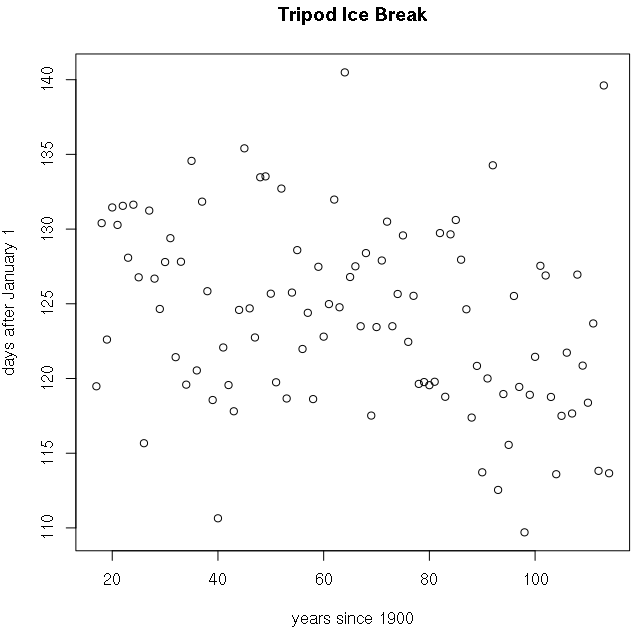
\includegraphics[scale=0.28]{./diagrams/nenana-01.png}
  \end{figure}
\end{frame}

\begin{frame}
  \frametitle{Hypothesis Testing in R}
  \begin{description}
  \item[Step 1] The null hypothesis is $\varrho=0$. The alternative
    hypothesis is $\varrho<0$ (the Earth is warming, therefore the
    tripod will break up the ice earlier in the year the more recently
    we measure). We will test the null hypothesis at a significance
    level of $\alpha=0.01$.
  \item[Step 2] The test statistic is $r=-0.3130899$ (calculated using
    R Statistics).
  \item[Step 3] The critical value of the Pearson Correlation
    Coefficient $r$ is approximately $0.256$ at $\alpha=0.01$ and
    $n=98$ (consult the table).
  \end{description}
  Decision: reject the null hypothesis. The data supports the
  hypothesis that there is a linear correlation between years after
  1900 and the days after January 1 when the tripod breaks the ice
  (assuming that the data have a bivariate normal distribution and a
  linear rather than some other correlation). 
\end{frame}

\begin{frame}[fragile,fragile]
  \frametitle{Hypothesis Testing in R}
  Here is how you can do the hypothesis testing in R Statistics.
  Let $y$ be the years after 1900 and $d$ be the days after January 1
  when the tripod breaks the ice. Try the command
  \texttt{summary(lm(d~y))}. The output is on the next slide. Notice
  the $p$-value. It clearly suggests that we should reject $H_{0}$.
\end{frame}

\begin{frame}[fragile,fragile]
  \frametitle{Hypothesis Testing in R}
\begin{verbatim}
Residuals:
     Min       1Q   Median       3Q      Max 
-15.2035  -3.6805  -0.2056   4.0684  18.7533 

Coefficients:
             Estimate Std. Error t value Pr(>|t|)    
(Intercept) 128.58108    1.50954   85.18   <2e-16 ***
y            -0.06834    0.02116   -3.23   0.0017 ** 
---
Signif. codes:  0 ‘***’ 0.001 ‘**’ 0.01 ‘*’ 0.05 ‘.’ 0.1 ‘ ’ 1

Residual standard error: 5.925 on 96 degrees of freedom
Multiple R-squared:  0.09803,	Adjusted R-squared:  0.08863 
F-statistic: 10.43 on 1 and 96 DF,  p-value: 0.001695
\end{verbatim}
\end{frame}

\begin{frame}
  \frametitle{Hypothesis Testing in R}
  Let's have a closer look at the summary on the last slide. The
  \alert{residuals} are the errors of our predictions using the
  regression line. For each $x$-value (independent variable), there is
  a $y$-value (dependent variable) and a $\hat{y}$-value (prediction
  using the regression line. The residual is $\hat{y}-y$ (in R
  Statistics, the residuals are in \texttt{z[[3]]} for
  \texttt{z<-summary(lm(d~y))}). The residual standard deviation
  $s_{e}$ is a measure how much the data scatters along the regression
  line:
  \begin{equation}
    \label{eq:eilokaqu}
    s_{e}=\sqrt{\frac{\sum(\hat{y}-y)^{2}}{n-2}}
  \end{equation}
  The residual standard deviation for the Nenana data is large, 5.925
  days, because even if you know the regression line it's hard to
  predict the date when the ice will be broken in a particular year.
\end{frame}

\begin{frame}
  \frametitle{Hypothesis Testing in R}
  $s_{e}$ is one measure of the relationship between $x$-values and
  $y$-values. The correlation coefficient $r$ is another one. In the R
  summary it is called ``Multiple R-squared'' and equals $r^{2}$. The
  reason why it is squared is because one could say that the
  correlation accounts for $r^{2}$ of the variation in the $y$-values.
  In the Nenana example, which year it is accounts for 9.8\% of the
  variation in the number of days it takes for the ice to break.

  \bigskip

  Some statisticians prefer ``Adjusted R-squared'' which penalizes
  larger numbers of parameters.
\end{frame}

\begin{frame}
  \frametitle{Hypothesis Testing in R}
  A theorem in statistics tells us that
  \begin{equation}
    \label{eq:aekeeque}
    \frac{b_{1}-\beta_{1}}{\frac{s_{e}}{s_{x}\sqrt{n-1}}}
  \end{equation}
  is distributed according to a $t$-distribution with degree of
  freedom $df=n-2$. 
\end{frame}

\begin{frame}
  \frametitle{Hypothesis Testing in R}
  $s_{x}$ is the standard deviation of the $x$-values. $s_{e}$ is the
  residual standard deviation. $b_{1}$ is the slope of the regression
  line calculated from the sample; $\beta_{1}$ is the slope of the
  regression line hypothesized for the population.

  \bigskip
  
  The R summary tells us that the slope of the regression line for the
  sample is $b_{1}=-0.06834$ and the $p$-value for the hypothesis that
  $\beta_{1}=0$ is $0.0017$ (two-tailed) (you can check this by
  looking at the $t$-distribution with degree of freedom $df=96$ and
  the result of the formula on the last slide, which is
  $t^{\ast}=-3.23$). We reject the hypothesis that $\beta_{1}=0$,
  which is similar to rejecting the hypothesis that $r=0$. It is
  usually not interesting to investigate the hypothesis that the
  $y$-intercept is zero.
\end{frame}

\begin{frame}
  \frametitle{Hypothesis Testing in R}
  Here is yet another hypothesis test whether there is a linear
  correlation or not. A relatively complicated formula gives us the
  \alert{F-statistic} of the regression analysis. The F-distribution
  (named after Ronald Fisher) looks similar to the chi-squared
  distribution. It has two degrees of freedom. In R Statistics,
  \texttt{qf(0.95,5,2)} gives you the F-statistic for which 95\% of
  the area under the curve is to the left of the F-statistic, with
  degrees of freedom 5 and 2. \texttt{pf(19.29641,5,2)} is the reverse
  procedure which gives you the area under the curve to the left of
  the F-statistic $19.29641$. We will meet this distribution again
  when we cover ANOVA.
\end{frame}

\begin{frame}[fragile]
  \frametitle{Hypothesis Testing for Correlation Exercise}
  {\ubung} The table below lists measured amounts of redshift and
  the distances (billions of light-years) to randomly selected
  clusters of galaxies. Is there sufficient evidence to conclude
  that there is a linear correlation between amounts of redshift
  and distances to clusters of galaxies?
  \begin{footnotesize}
\begin{verbatim}
+----------+----------+
| Redshift | Distance |
+----------+----------+
|   0.0233 |     0.32 |
+----------+----------+
|   0.0539 |     0.75 |
+----------+----------+
|   0.0718 |     1.00 |
+----------+----------+
|   0.0395 |     0.55 |
+----------+----------+
|   0.0438 |     0.61 |
+----------+----------+
|   0.0103 |     0.14 |
+----------+----------+
\end{verbatim}
  \end{footnotesize}
  % Redshift,Distance
  % 0.0233,0.32
  % 0.0539,0.75
  % 0.0718,1.00
  % 0.0395,0.55
  % 0.0438,0.61
  % 0.0103,0.14
\end{frame}

\begin{frame}
  \frametitle{The Regression Line}
  To find the regression line $\hat{y}=b_{0}+b_{1}x$, use the
  following formula for the slope $b_{1}$ and the $y$-intercept
  $b_{0}$:
  \begin{equation}
    \label{eq:ohzashur}
    b_{1}=\frac{n\left(\sum{}xy\right)-\left(\sum{}x\right)\left(\sum{}y\right)}{n\left(\sum{}x^{2}\right)-\left(\sum{}x\right)^{2}}
  \end{equation}
  \begin{equation}
    \label{eq:xuothaba}
    b_{0}=\frac{\left(\sum{}y\right)\left(\sum{}x^{2}\right)-\left(\sum{}x\right)\left(\sum{}xy\right)}{n\left(\sum{}x^{2}\right)-\left(\sum{}x\right)^{2}}
  \end{equation}
 You may wonder where these equations come from. They identify the
 line equation which best fits the data using the \alert{least
   squares} method. The least squares method identifies the line
 that best fits the data by measuring the distance that each data
 point is away from the line, squaring it, and then adding all of
 those numbers. The line that scores lowest on this fitness test
 is the regression line.
\end{frame}

\begin{frame}
  \frametitle{Regression Line Example}
  \beispiel{Galaxy Distances} It is clear in the hypothesis test
  that there is a linear correlation between redshift and galaxy
  distances, even with a small sample size. What is the regression
  line? How could we predict the distance of a galaxy, knowing its
  redshift?
  \begin{equation}
    \label{eq:ahnuwiez}
    \begin{array}{rcl}
      b_{0}&=&-0.004396 \\
      b_{1}&=&13.999899
    \end{array}
  \end{equation}
  Each thousandth unit of redshift adds fourteen million light-years to
  the distance.

  \bigskip

  In R Statistics, you can create a scatterplot of data sets
  \texttt{x} and \texttt{y} using the command \texttt{plot(x,y)}.
  Adding the command \texttt{abline(lm(y}$\sim$\texttt{x),col="red")} will add
  the regression line to the plot (in red colour).
  \texttt{lm(y}$\sim$\texttt{x)} will give you both the $y$-intercept and the
  slope of the regression line.
\end{frame}

\begin{frame}[fragile]
  \frametitle{Regression Line Example}
  Here is some R Statistics code:
\begin{alltt}
a<-runif(500,0,1) \newline
b<-rnorm(500,a,0.2) \newline
plot(a,b) \newline
abline(lm(b~a),col="red")
\end{alltt}
\end{frame}

\begin{frame}
  \frametitle{Regression Line Example}
  \begin{figure}[h]
    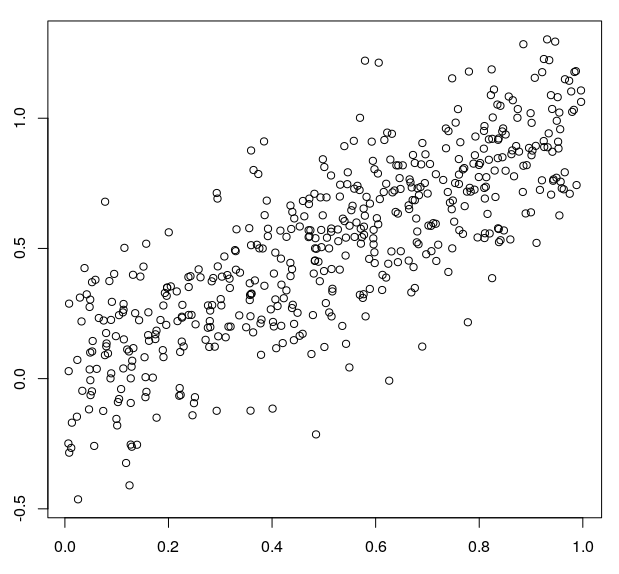
\includegraphics[scale=0.4]{./diagrams/abline1.png}
  \end{figure}
\end{frame}

\begin{frame}
  \frametitle{Regression Line Example}
  \begin{figure}[h]
    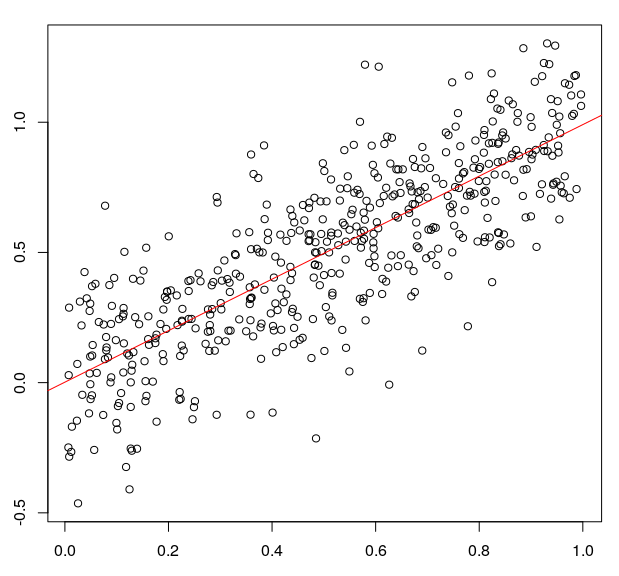
\includegraphics[scale=0.4]{./diagrams/abline2.png}
  \end{figure}
\end{frame}

\begin{frame}
  \frametitle{Regression Line Exercise}
  {\ubung} Consider the data on the next slide. These are the
  results for two successive term tests (the names are randomly
  made up by a computer program, but the grades are real). Answer
  the following questions:
  \begin{enumerate}
  \item Is there a linear correlation between the first and the
    second term test? Answer the question for a significance level
    of $\alpha=0.05$. If you were doing this problem with a
    significance level $\alpha=0.01$, what would be the decision
    and what type of error (type I or type II) would it make less
    likely compared to using the higher significance level?
  \item What is the equation of the regression line?
  \item If William Jones (again, fake name but real grade) had a
    score of $85$ on the first term test, what score is the point
    estimate for the second term test given the linear
    correlation? His true score for the second term test was $77$.
  \end{enumerate}
% Nancy Rogge,83,60,,Arnold Murray,73,82
% Elizabeth Rushing,98,95,,Ann Coburn,60,52
% Katy Nunez,68,62,,Kim Lazzari,63,62
% Michael Preuss,68,90,,Valentina Martinez,68,88
% Edna Phipps,68,90,,Eric Mumford,78,91
% George Thompson,45,85,,Alyssa Warner,98,90
% James Newman,42,20,,Kevin Ellis,65,72
% Nathan Stowman,108,90,,Susan Ervin,90,80
% Kimberly Gaitor,83,90,,Albert Gutierrez,55,52
% Leland Garner,60,65,,Robin Calderon,95,100
% Bryan Veilleux,53,75,,Jennifer Blackburn,60,57
% Mary Watts,73,86,,Doris Larkin,83,85
% Jerry Brown,58,60,,James Miller,63,42
% Jacob Ludwick,47,52,,Gregory Myklebust,70,87
% Wayne Vega,100,85,,Rita Swinton,90,90
% Kathryn Wilson,55,80,,Barbara Richardson,63,82
% Tony Bateman,20,11,,Ora Tidmore,108,87
\end{frame}

\begin{frame}
  \frametitle{Regression Line Exercise}
% +--------------------+----+----++--------------------+-----+----+ \newline
% |    Nancy Rogge     | 83 | 60 ||   Arnold Murray    |  73 | 82 | \newline
% +--------------------+----+----++--------------------+-----+----+ \newline
% | Elizabeth Rushing  | 98 | 95 ||     Ann Coburn     |  60 | 52 | \newline
% +--------------------+----+----++--------------------+-----+----+ \newline
% |     Katy Nunez     | 68 | 62 ||    Kim Lazzari     |  63 | 62 | \newline
% +--------------------+----+----++--------------------+-----+----+ \newline
% |   Michael Preuss   | 68 | 90 || Valentina Martinez |  68 | 88 | \newline
% +--------------------+----+----++--------------------+-----+----+ \newline
% |    Edna Phipps     | 68 | 90 ||    Eric Mumford    |  78 | 91 | \newline
% +--------------------+----+----++--------------------+-----+----+ \newline
% |  George Thompson   | 45 | 85 ||   Alyssa Warner    |  98 | 90 | \newline
% +--------------------+----+----++--------------------+-----+----+ \newline
% |    James Newman    | 42 | 20 ||    Kevin Ellis     |  65 | 72 | \newline
% +--------------------+----+----++--------------------+-----+----+ \newline
% |   Nathan Stowman   | 08 | 90 ||    Susan Ervin     |  90 | 80 | \newline
% +--------------------+----+----++--------------------+-----+----+ \newline
% |  Kimberly Gaitor   | 83 | 90 ||  Albert Gutierrez  |  55 | 52 | \newline
% +--------------------+----+----++--------------------+-----+----+ \newline
% |   Leland Garner    | 60 | 65 ||   Robin Calderon   |  95 | 00 | \newline
% +--------------------+----+----++--------------------+-----+----+ \newline
% |   Bryan Veilleux   | 53 | 75 || Jennifer Blackburn |  60 | 57 | \newline
% +--------------------+----+----++--------------------+-----+----+ \newline
% |     Mary Watts     | 73 | 86 ||    Doris Larkin    |  83 | 85 | \newline
% +--------------------+----+----++--------------------+-----+----+ \newline
% |    Jerry Brown     | 58 | 60 ||    James Miller    |  63 | 42 | \newline
% +--------------------+----+----++--------------------+-----+----+ \newline
% |   Jacob Ludwick    | 47 | 52 || Gregory Myklebust  |  70 | 87 | \newline
% +--------------------+----+----++--------------------+-----+----+ \newline
% |     Wayne Vega     | 00 | 85 ||    Rita Swinton    |  90 | 90 | \newline
% +--------------------+----+----++--------------------+-----+----+ \newline
% |   Kathryn Wilson   | 55 | 80 || Barbara Richardson |  63 | 82 | \newline
% +--------------------+----+----++--------------------+-----+----+ \newline
% |    Tony Bateman    | 20 | 11 ||    Ora Tidmore     | 108 | 87 | \newline
% +--------------------+----+----++--------------------+-----+----+
% This LaTeX table template is generated by emacs 24.5.1
  \begin{footnotesize}
\begin{tabular}{|l|l|l|l|l|l|l|}
\hline
Nancy Rogge & 83 & 60 & & Arnold Murray & 73 & 82 \\
\hline
Elizabeth Rushing & 98 & 95 & & Ann Coburn & 60 & 52 \\
\hline
Katy Nunez & 68 & 62 & & Kim Lazzari & 63 & 62 \\
\hline
Michael Preuss & 68 & 90 & & Valentina Martinez & 68 & 88 \\
\hline
Edna Phipps & 68 & 90 & & Eric Mumford & 78 & 91 \\
\hline
George Thompson & 45 & 85 & & Alyssa Warner & 98 & 90 \\
\hline
James Newman & 42 & 20 & & Kevin Ellis & 65 & 72 \\
\hline
Nathan Stowman & 108 & 90 & & Susan Ervin & 90 & 80 \\
\hline
Kimberly Gaitor & 83 & 90 & & Albert Gutierrez & 55 & 52 \\
\hline
Leland Garner & 60 & 65 & & Robin Calderon & 95 & 100 \\
\hline
Bryan Veilleux & 53 & 75 & & Jennifer Blackburn & 60 & 57 \\
\hline
Mary Watts & 73 & 86 & & Doris Larkin & 83 & 85 \\
\hline
Jerry Brown & 58 & 60 & & James Miller & 63 & 42 \\
\hline
Jacob Ludwick & 47 & 52 & & Gregory Myklebust & 70 & 87 \\
\hline
Wayne Vega & 100 & 85 & & Rita Swinton & 90 & 90 \\
\hline
Kathryn Wilson & 55 & 80 & & Barbara Richardson & 63 & 82 \\
\hline
Tony Bateman & 20 & 11 & & Ora Tidmore & 108 & 87 \\
\hline
\end{tabular}
  \end{footnotesize}
\end{frame}

\begin{frame}
  \frametitle{Regression Line Exercise}
  \begin{tabular}{|l|r|l|r|}\hline
    \hspace{.5in} & & & \\
    $\sum{}x$ & $2496$ & $\sum{}y$ & $2580$ \\
    \hspace{.5in} & & & \\ \hline
    \hspace{.5in} & & & \\
    $\sum{}x^{2}$ & $191344$ & $\sum{}y^{2}$ & $204700$ \\
    \hspace{.5in} & & & \\ \hline
    \hspace{.5in} & & & \\
    $\left(\sum{}x\right)^{2}$ & $6230016$ & $\left(\sum{}y\right)^{2}$ & $6656400$ \\
    \hspace{.5in} & & & \\ \hline
    \hspace{.5in} & & & \\
    $\sum{}xy$ & $193904$ & $n$ & $34$ \\
    \hspace{.5in} & & & \\ \hline
  \end{tabular}
\end{frame}

\begin{frame}
  \frametitle{Regression Line Exercise}
  The solution for the linear correlation coefficient is
  $r=0.7122366$.

  \bigskip

  The solution for the $y$-intercept and slope of the regression
  line is $b_{0}=20.7350$ and $b_{1}=0.7429$. The point estimate
  for William Jones' grade is $83.88$.
\end{frame}

\begin{frame}
  \frametitle{Regression Line Exercise}
  \begin{figure}[h]
    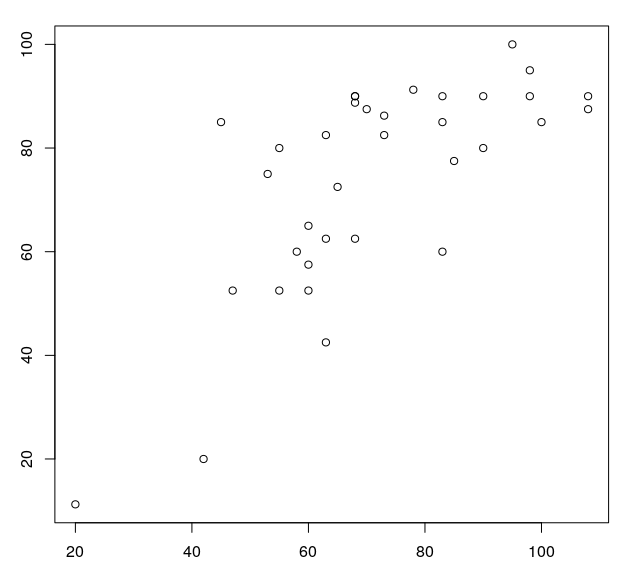
\includegraphics[scale=0.4]{./diagrams/grades1.png}
  \end{figure}
\end{frame}

\begin{frame}
  \frametitle{Regression Line Exercise}
  \begin{figure}[h]
    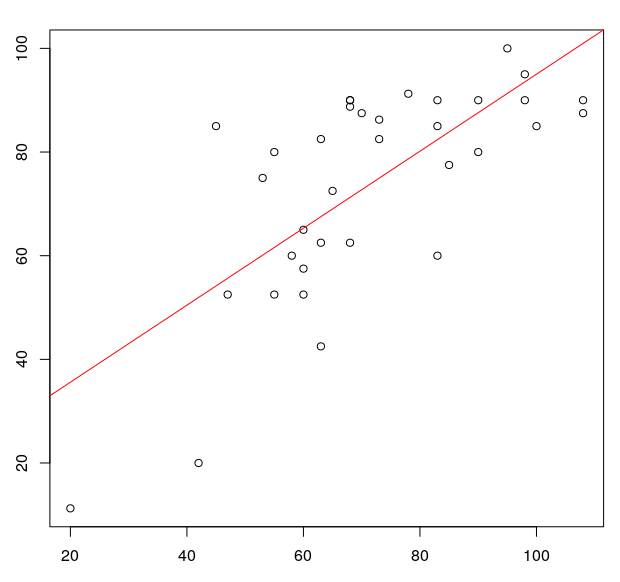
\includegraphics[scale=0.4]{./diagrams/grades2.png}
  \end{figure}
\end{frame}

\begin{frame}
  \frametitle{Linear Correlation Exercise}
Costs listed below are repair costs (in dollars) for cars crashed
at 6 mi/h in full-front crash tests and the same cars crashed at 6
mi/h in full-rear crash tests (based on data from the Insurance
Institute for Highway Safety). The cars are the Toyota Camry,
Mazda 6, Volvo S40, Saturn Aura, Subaru Legacy, Hyundai Sonata,
and Honda Accord. Is there sufficient evidence to conclude that
there is a linear correlation between the repair costs from
full-front crashes and full-rear crashes?

\bigskip

% This LaTeX table template is generated by emacs 24.5.1
\begin{tabular}{|l|l|l|l|l|l|l|l|}
\hline
Front & 936 & 978 & 2252 & 1032 & 3911 & 4312 & 3469 \\
\hline
Rear & 1480 & 1202 & 802 & 3191 & 1122 & 739 & 2767 \\
\hline
\end{tabular}
% +---------+---------+---------+---------+---------+---------+---------+---------+
% |  Front  |   936   |   978   |  2252   |  1032   |  3911   |  4312   |  3469   |
% +---------+---------+---------+---------+---------+---------+---------+---------+
% |  Rear   |  1480   |  1202   |   802   |  3191   |  1122   |   739   |  2767   |
% +---------+---------+---------+---------+---------+---------+---------+---------+

% Front,936,978,2252,1032,3911,4312,3469
% Rear,1480,1202,802,3191,1122,739,2767
\end{frame}

\begin{frame}
  \frametitle{Linear Correlation Exercise}
  Listed below are systolic blood pressure measurements (in mm Hg)
  obtained from the same woman (based on data from ``Consistency of
  Blood Pressure Differences Between the Left and Right Arms,'' by
  Eguchi et al., Archives of Internal Medicine, Vol.\ 167). Is there
  sufficient evidence to conclude that there is a linear correlation
  between right and left arm systolic blood pressure measurements?

% +---------------+---------------+---------------+---------------+---------------+---------------+
% |Right Arm      |102            |101            |94             |79             |79             |
% +---------------+---------------+---------------+---------------+---------------+---------------+
% |Left Arm       |175            |169            |182            |146            |144            |
% +---------------+---------------+---------------+---------------+---------------+---------------+

\bigskip

% This LaTeX table template is generated by emacs 24.5.1
\begin{tabular}{|l|l|l|l|l|l|}
\hline
Right Arm & 102 & 101 & 94 & 79 & 79 \\
\hline
Left Arm & 175 & 169 & 182 & 146 & 144 \\
\hline
\end{tabular}

% Right Arm,102,101,94,79,79
% Left Arm,175 ,169,182,146,144
\end{frame}

\begin{frame}
  \frametitle{Linear Correlation Exercise}
  One classic application of correlation involves the association
  between the temperature and the number of times a cricket chirps in
  a minute. Listed below are the numbers of chirps in one minute and the
  corresponding temperatures in $^{\circ}$F (based on data from ``The Song of
  Insects'' by George W. Pierce, Harvard University Press). Is there
  sufficient evidence to conclude that there is a linear correlation
  between the number of chirps in one minute and the temperature?

% This LaTeX table template is generated by emacs 24.5.1
\bigskip

\begin{tabular}{|l|l|l|l|l|l|l|l|l|}
\hline
Chirps & 882 & 1188 & 1104 & 864 & 1200 & 1032 & 960 & 900 \\
\hline
$^{\circ}$F & 69.7 & 93.3 & 84.3 & 76.3 & 88 6 & 82.6 & 71.6 & 79.6 \\
\hline
\end{tabular}

% +---------+---------+---------+---------+---------+---------+---------+---------+---------+
% |000      |882      |1188     |1104     |864      |1200     |1032     |960      |900      |
% +---------+---------+---------+---------+---------+---------+---------+---------+---------+
% |000      |69.7     |93.3     |84.3     |76.3     |88 6     |82.6     |71.6     |79.6     |
% +---------+---------+---------+---------+---------+---------+---------+---------+---------+
\end{frame}

% 25.	Gas Prices Gas prices have been very volatile in recent years. The table below lists gas prices (dollars per gallon) at randomly selected Connecticut stations at the time of this writing (based on data from AOL Autos). Is there sufficient evidence to conclude that there is a linear correlation between prices of regular gas and prices of premium gas? For the gas stations that sometimes post only the price of regular gas, can you use those prices to get a good sense of the price of premium gas?
% Regular	2.77	2.77	2.79	2.81	2.78	2.86	2.75	2.77
% Mid-Grade	3.00	2.77	2.89	2.93	2 93	2.96	2.86	2.91
% Premium	3.07	3.09	3.00	3.06	3.03 	—	3.06	3.02	3.03

% 26.	Gas Prices Repeat the preceding exercise using the prices of regular gas and the prices of mid-grade gas.

% 27.	Sports Diameters (cm), circumferences (cm), and volumes (cm3) from balls used in different sports are listed in the table below. Is there sufficient evidence to conclude that there is a linear correlation between diameters and circumferences? Docs the scattcrplot confirm a linear association?

\begin{frame}
  \frametitle{Linear Correlation Exercise}
  Lemons and Car Crashes. Find the best predicted crash fatality rate
  for a year in which there are 500 metric tons of lemon imports.

% +---------+---------+---------+---------+---------+---------+
% |000      |230      |265      |358      |480      |530      |
% +---------+---------+---------+---------+---------+---------+
% |000      |15.9     |15.7     |15.4     |15.3     |14.9     |
% +---------+---------+---------+---------+---------+---------+

  \bigskip

% This LaTeX table template is generated by emacs 24.5.1
\begin{tabular}{|l|l|l|l|l|l|}
\hline
Lemon Imports & 230 & 265 & 358 & 480 & 530 \\
\hline
Crash Fatality Rate & 15.9 & 15.7 & 15.4 & 15.3 & 14.9 \\
\hline
\end{tabular}
\end{frame}

% 14.	PSAT and SAT Scores One subject not included in the given table had a PSAT score of 229. Find the best predicted SAT score for this student. Is the result close to the reported value of 2400? Given that the data arc from volunteered responses, are the results valid?
% PSAT	183	207	167	206	197	142	193	176
% SAT	2200	2040	1890	2380	2290	2070	2370	1980

% 15.	Campus Crime Find the best predicted number of burglaries for Ohio State, which had an enrollment of 51,800 students. Is the predicted value close to 329, which was the actual number of burglaries?
% Enrollment	32	31	53	28	27	36	I 42 I	30	34	46
% Burgla'ies	103	103	86	57	32	131	: 157 j	20	27	161

\begin{frame}
  \frametitle{Linear Correlation Exercise}
  Altitude and Temperature. At 6327 ft (or 6.327 thousand feet), Mario
  Triola, the author of many of these exercises, recorded the
  temperature. Find the best predicted temperature at that altitude.
  How does the result compare to the actual recorded value of 48$^{\circ}$F?

% +---------+---------+---------+---------+---------+---------+---------+---------+
% |000      |3        |10       |14       |22       |28       |31       |33       |
% +---------+---------+---------+---------+---------+---------+---------+---------+
% |000      |57       |37       |24       |-5       |-30      |-41      |-54      |
% +---------+---------+---------+---------+---------+---------+---------+---------+

  \bigskip

% This LaTeX table template is generated by emacs 24.5.1
\begin{tabular}{|l|l|l|l|l|l|l|l|}
\hline
Altitude & 3 & 10 & 14 & 22 & 28 & 31 & 33 \\
\hline
Temperature & 57 & 37 & 24 & -5 & -30 & -41 & -54 \\
\hline
\end{tabular}
% Altitude	3	10	14	22	28	31	33
% Temperature	57	37	24	-5	-30	-41	-54
\end{frame}


% 17. Town Courts The court for the town of Beckman had income of $83,941 (or $83,941 thousand). Find the best predicted salary for the justice. Is the result close to the actual salary of $26,088?
% Court Income	65	404	1567	1131	272	252	111	154	32
% Justice Salary	30	j 44	92	56	46	61	25	26	18

% 18. Auction Bids An item not included in the table is a pair of New York Knicks tickets. The auctioneer started the bidding at $300. Find the best predicted winning bid. Is the result close to the actual winning bid of $250?
% Opening Bid	1500	500	500	400	j 300
% Winning Bid	650	175	125	275	125

\begin{frame}
  \frametitle{Confidence Interval for Regression Line Slope}
  If the regression line slope for a sample of size $n$ is $b_{1}$,
  then a confidence interval for the regression line slope $\beta_{1}$
  of the population is (the confidence level being $1-\alpha$)
  \begin{equation}
    \label{eq:ooghiech}
    b_{1}-E<\beta_{1}<b_{1}+E
  \end{equation}
  with
  \begin{equation}
    \label{eq:ongiemas}
    % E=t_{\frac{\alpha}{2}}\frac{s_{e}\sqrt{\sum{}x^{2}}}{\sqrt{n}\left(\sum{}x^{2}-\frac{\left(\sum{}x\right)^{2}}{n}\right)}
    E=t_{\frac{\alpha}{2}}\frac{s_{e}}{s_{x}\sqrt{n-1}}
  \end{equation}
  The degree of freedom for $t_{\frac{\alpha}{2}}$ is $n-2$.
\end{frame}

\begin{frame}
  \frametitle{Confidence Interval for Regression Line Slope}
  The data on the next slide shows observations of the Old Faithful
  geyser in the USA Yellowstone National Park. There are two
  observation variables in the data set. The first one, called
  eruptions, is the duration of the geyser eruptions. The second one,
  called waiting, is the length of waiting period until the next
  eruption (all in minutes). It turns out there is a correlation
  between the two variables. The data is available on R Statistics in
  the dataframe called \texttt{faithful}.
\end{frame}

\begin{frame}
  \frametitle{Confidence Interval for Regression Line Slope}
\begin{figure}[h]
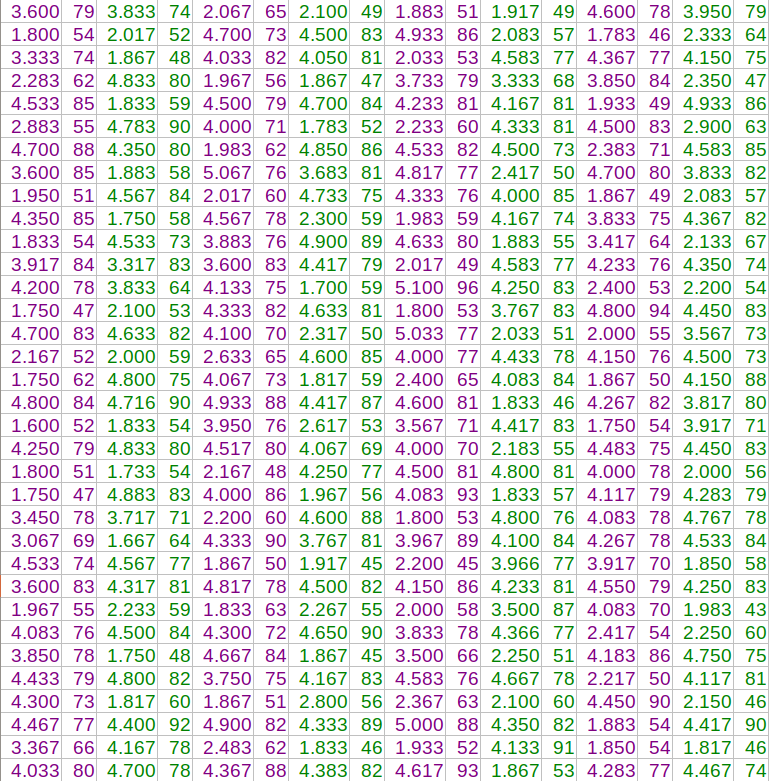
\includegraphics[scale=.35]{./diagrams/faithful.png}
\end{figure}
\end{frame}

\begin{frame}
  \frametitle{Confidence Interval for Regression Line Slope}
  For the data on the last slide, the residual standard error
  $s_{e}=5.914$. The regression line for the sample is
  \begin{equation}
    \label{eq:eiheelut}
    \hat{y}=33.4744+10.7296x
  \end{equation}
These numbers were gathered from the R Statistics command
\texttt{summary(lm(faithful[[2]]~faithful[[1]]))}. 
\end{frame}

\begin{frame}
  \frametitle{Confidence Interval for Regression Line Slope}
  The error for the 95\% confidence interval is
  of 
\begin{equation}
  \label{eq:gaeyiegh}
% E=t_{\frac{\alpha}{2}}\frac{s_{e}\sqrt{\sum{}x^{2}}}{\sqrt{n}\left(\sum{}x^{2}-\frac{\left(\sum{}x\right)^{2}}{n}\right)}=\notag
E=t_{\frac{\alpha}{2}}\frac{s_{e}}{s_{x}\sqrt{n-1}}=\notag
\end{equation}
\begin{equation}
  \label{eq:eevievuo}
  % 1.968789\cdot\frac{5.914\cdot{}60.51297}{\sqrt{272}\cdot\left(3661.819-\frac{899988.1}{272}\right)}=0.12101
  1.968789\cdot\frac{5.914}{3.4878\sqrt{272-1}}=0.61968
\end{equation}

Consequently, the confidence interval
\begin{equation}
  \label{eq:sahshixu}
  b_{1}-E<\beta_{1}<b_{1}+E
\end{equation}
is $(10.10996,11.34932)$
The R Statistics command \texttt{confint(lm(y~x),'x',level=0.95)} will
give you the same result.
\end{frame}

\begin{frame}
  \frametitle{Prediction Interval for Linear Regression}
  We already know how to predict the dependent variable (in this case,
  the waiting time for the next geyser) if we know the independent
  variable (in this case, the eruption time). For example, if the
  eruption time is four minutes (which happens to be the median of the
  data set), then the point estimate for the waiting time is
  \begin{equation}
    \label{eq:thaejola}
    \hat{y}=33.4744+10.7296\cdot{}4=76.3928
  \end{equation}
What is the confidence interval around this point estimate, again at a
confidence level of $1-\alpha=0.95$? The error in this case is
\begin{equation}
  \label{eq:suquiequ}
  E=t_{\frac{\alpha}{2}}s_{e}\sqrt{1+\frac{1}{n}+\frac{(x-\bar{x})^{2}}{\sum{}x^{2}-\frac{\left(\sum{}x\right)^{2}}{n}}}
\end{equation}
\end{frame}

\begin{frame}
  \frametitle{Prediction Interval for Linear Regression}
  Plugging in the numbers from the faithful example, the confidence
  interval
  \begin{equation}
    \label{eq:miiniphu}
    \bar{y}-E<y<\bar{y}+E
  \end{equation}
  is $(64.72368,88.06192)$.

  \bigskip

  The R Statistics command \texttt{predict(lm(y{\texttildelow}x),data.frame(x=4.5),level=0.95,interval="predict")}
  will give you the same result.
\end{frame}

% \begin{frame}[fragile,fragile]
%   \frametitle{In R Statistics}
%   In R Statistics, you can find the confidence interval for the slope
%   of the regression line as follows,
% \begin{alltt}
% confint(lm(faithful[[2]]~faithful[[1]]),'faithful[[1]]',level=0.95)
% \end{alltt}
%   You can find the confidence interval of the prediction for the
%   waiting time as follows, assuming that the eruption lasted for four
%   minutes,
% \begin{alltt}

% \end{alltt}
% \end{frame}

\begin{frame}
  \frametitle{Flow Chart for Linear Regression Hypothesis Testing}
\begin{figure}[h]
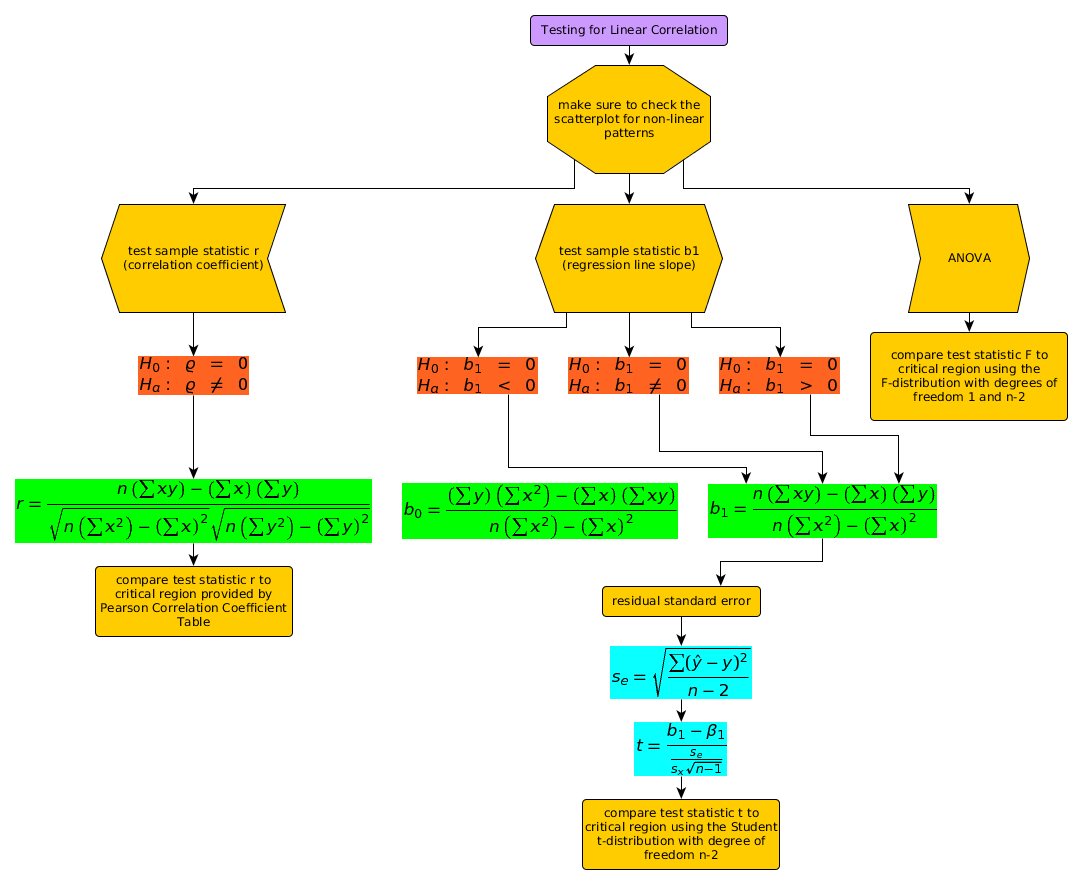
\includegraphics[scale=.24]{./diagrams/linear-regression.png}
\end{figure}
\end{frame}

\begin{frame}
  \frametitle{End of Lesson}
Next Lesson: Goodness of Fit
\end{frame}

\end{document}

